\exercice{Corde vibrante conductrice}
On étudie les petits mouvements transversaux d'une corde métallique de longueur $L$ fixée en ses extrémités d'abscisse $x=0$ et $x=L$. Un point de la corde, situé à l'abscisse $x$ à la date $t$ au repos, se déplace de $z(x,t)$ au passage de l'onde. On néglige la pesanteur. La corde est parcourue par un courant d'intensité $i(t)=i_0\cos(\omega t)$ et plongée dans un champ magnétique $\vv{B}(x)=B_0\sin(\frac{\pi x}{L})\vv{u_y}$. On rappelle que la force de Laplace qui s'exerce sur un élément de longueur $\vv{dl}$ est $\vv{df}=i\vv{dl}\wedge\vv{B}$.
\begin{enumerate}
  \question{Établir l'équation du mouvement de la corde sous la forme
  $\frac{\partial^2 z}{\partial t^2}-c^2\frac{\partial^2 z}{\partial x^2}=\frac{i_0 B_0}{\mu}\cos(\omega t)\sin(\frac{\pi x}{L})$
  où $c$ est une constante à exprimer en fonction des données de l'énoncé.}
    [Reprendre la démonstration de l'équation de d'Alembert avec cette fois-ci la force de Laplace en plus.]
  \question{On cherche une solution en $z(x,t)=z_0\sin(\frac{\pi x}{L})\cos(\omega t)$ en régime sinusoïdal forcé. Commenter le choix de cette expression.}
    [Cette onde est-elle une onde stationnaire ou progressive ?]
    [Le milieu est-il fini, semi-infini ou infini ?]
  \question{Déterminer l'expression de $z_0$. Que se passe-t-il quand $\omega$ tend vers $\frac{\pi c}{L}$ ? La modélisation du phénomène est-elle toujours valable ? Expliquer.}
    [Introduire l'expression de $z$ dans l'équation d'onde.]
    [Les hypothèses faire pour établir l'équation d'onde sont-elles compatibles avec une amplitude qui diverge ?]
\end{enumerate}

\exercice{Câble coaxial alimenté par un générateur}
A coaxial line of length $L$ is powered at one end by a voltage source $e(t)=E_0\cos(\omega t)$. The other end is left open.
\begin{enumerate}
  \question{Ascertain the voltage wave $u(x,t)$ and the current wave $i(x,t)$.}
    [Deux possibilités : soit chercher les solutions sous la forme $f(x)g(t)$ (milieu fini), soit sous la forme d'une onde incidente plus une onde réfléchie.]
    [Quelles sont les conditions aux limites en $x=0$ ? en $x=L$ ?]
  \question{For some values of $\omega$, the amplitude of $u$ and $i$ are very important. Explain why and for determine the values of $\omega$ for which this happens.}
\end{enumerate}


\exercice{Modèle d'une clarinette}
Une clarinette est modélisée par un tuyau de section $S$ et de longueur $l$. Il contient un fluide pour lequel la célérité des ondes sonores est $c$. Une extrémité du tuyau est fixe alors que l'autre est ouverte sur l'atmosphère, qui y impose la pression $P_0$. Ce modèle simpliste permet d'aboutir aux fréquences émises par l'instrument, il s'applique aussi au saxophone, basson, tuyau d'orgue, \dots{}.
\begin{figure}[!ht]
  \centering
  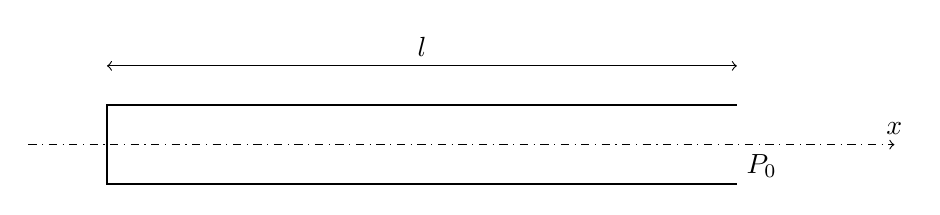
\begin{tikzpicture}
  \draw[dashdotted,->] (-1,0) -- (10,0) node[above] {$x$};
  \draw[thick] (8,0.5) -- (0,0.5) -- (0,-0.5) -- (8,-0.5);
  \draw[<->] (0,1) -- (8,1) node[midway, above] {$l$};
  \draw (8,0) node[below right] {$P_0$};
\end{tikzpicture}
  

    
  
\end{figure}

Au repos, la pression vaut $P_0$ et la masse volumique $\rho_0$ dans le fluide de la flute. Les effets de la pesanteur sont négligés. On se place dans l'approximation acoustique.

Le musicien injecte à une extrémité du tuyau une onde sonore plane, il s'établit alors une onde stationnaire modélisée par l'onde de surpression $P_1(x,t)=A_0\cos(\omega t)\cos(kx)$.
\begin{enumerate}
  \question{Pourquoi modéliser l'onde sonore par une onde stationnaire ?}
    [Le milieu est-il fini, semi-infini ou infini ? Dans un tel milieu, sous quelle forme cherche-t-on des solutions de manière privilégiée ?]
  \question{Établir l'expression du champ de vitesse dans la clarinette. A-t-on $P_1(x,t)=Zv(x,t)$, où $Z=\rho_0c$ ?}
    [Écrire l'équation mécanique liant la surpression à la vitesse.]
  \question{Quelles sont les deux conditions aux limites imposées par l'atmosphère ?}
    [Attention, dans cet exercice, $P$ désigne la surpression et pas la pression comme dans le cours.]
    [Écrire la condition d'adhérence en $x=0$ et la continuité de la pression en $x=l$.]
  \question{Établir quelles pulsations peuvent être jouées avec cet instrument.}
    [Quelles valeurs de $k$ sont possible avec la condition aux limites sur la surpression en $x=l$ ?]
    [Relier $k$ à $\omega$ grâce à la relation de dispersion.]
  \question{La note fondamentale d'une flute de longueur $l$ est $\omega_f=\frac{\pi c}{l}$. Comparer la hauteur de son d'une flute et d'une clarinette de même longueur.}
    [La fondamentale est la plus petite fréquence ($n=1$).]
\end{enumerate}


\exercice{Modes propres dans une cavité sphérique}[1]
Un gaz est contenu à l'intérieur d'une sphère rigide de rayon $R$. Une onde sonore sphérique se propage dans la sphère, décrite par la surpression $P(r,t)$ et le champ des vitesse $v(r,t)\vv{u_r}$.

On se place dans le cas où $P(r,t)=\frac{A}{r}e^{j(\omega_1t-k_1r)}+\frac{B}{r}e^{j(\omega_2t+k_2r)}$.
\begin{enumerate}
  \question{Que représente chacun des termes de $P(r,t)$ ?}
    [Pour chaque terme, est-ce une onde stationnaire ou progressive . harmonique ou non ? sphérique, cylindrique ou plane ?]
  \question{Déterminer le champ des vitesses $\underline{v}$ associé à l'onde ?}
    [Attention, les ondes ne sont pas des OPPH, on ne peut pas utiliser l'impédance acoustique.]
    [Utiliser la relation mécanique liant la surpression et la vitesse.]
  \question{Établir le lien entre $\omega_1$ et $\omega_2$ puis $A$ et $B$. En déduire $\underline{v}$.}
    [Écrire la condition d'adhérence en $r=R$.]
    [Isoler les fonctions de $t$ d'un côté du signe égal.]
  \question{En supposant que la surpression ne diverge pas en $0$, montrer que $-2kR=\arctan\frac{2kR}{1-k^2R^2}$. Comment déterminer graphiquement les valeurs de $k$ possibles ?}
    % TO DO faire la résolution graphique ou avec Python.
    [Relier $A$ et $B$ simplement pour que la surpression ne diverge pas en 0.]
    [Reprendre la condition d'adhérence.]
    [Regrouper les exponentielles et appliquer la fonction argument.]
\end{enumerate}


\exercice{Cavité électromagnétique à une dimension}
On considère un espace vide compris entre deux plans infiniment conducteurs d'équation $x=0$ et $x=a$. On y étudie le champ électromagnétique.
\begin{enumerate}
  \question{Établir l'équation de propagation pour $\vv{E}$ dans le vide.}
  \question{On cherche des solutions à variables séparables : $\vv{E}=f(x)g(t)\vv{u_y}$. Établir les équations différentielles $f''(x)=\alpha f(x)$ et $g''(t)=\alpha c^2 g(t)$, où $\alpha$ est une constante inconnue à ce stade.}
    [Remplacer $\vv{E}$ par $f(x)g(t)\vv{e_y}$ dans l'équation de d'Alembert et séparer les variables.]
  \question{Quelles sont les conditions aux limites.}
    [Dans un conducteur parfait, le champ électrique est nul. De plus, la composante tangente à l'interface du champ électrique est continue.]
  \question{Déterminer $f(x)$. L'exprimer sous la forme d'une fonction de $kx$ où $k$ est une constante qui dépend de $\alpha$ et d'un entier $n$.}
    [L'équation différentielle sur $f$ a trois familles de solutions. Parmi elles, quelle est la seule admettant des solutions non nulles compatibles avec les conditions aux limites ?]
    [Quelle contrainte sur $k$ imposent les conditions aux limites ?]
  \question{En déduire l'expression de $\vv{E}$ en fonction de $k$ , d'une constante multiplicative près notée $E_0$ et d'une phase $\varphi$.}
    [Quelles sont les solutions de l'équation différentielle sur $g$ ?]
  \question{Quelle est l'analogue mécanique de ce problème électromagnétique ?}
    [Penser à un système où on a également des modes propres quantifiés à cause de deux conditions aux limites strictes.]
  \question{Établir l'expression du champ magnétique $\vv{B}$. Que dire des points où $\vv{B}$ est constamment nul, par rapport à ceux où $\vv{E}$ est constamment nul ?}
    [La relation de structure, démontrée pour une OPPH, ne peut pas être utilisée ici.]
    [Quelle équation de Maxwell permettrait de déterminer $\vv{B}$ ?]
    [Utiliser l'équation de Maxwell-Faraday.]
\end{enumerate}
